%        File: HW.tex
%     Created: 一 7月 02 01:00 下午 2018 C
% Last Change: 一 7月 02 01:00 下午 2018 C
%
\documentclass[UTF8,noindent]{ctexart}
\usepackage[a4paper,left=2.0cm,right=2.0cm,top=2.0cm,bottom=2.0cm]{geometry}
\usepackage{hyperref}
\usepackage{xeCJK}
\usepackage{url}
\usepackage{graphicx}
\usepackage{amsmath}
\usepackage{amssymb}
\usepackage{enumitem}
\usepackage{tikz,mathpazo}
\usetikzlibrary{shapes.geometric, arrows,calc}
\usepackage{float}
\usepackage{listings}
\usepackage{xcolor}
\lstset{language = c,numbers=left, keywordstyle= \color{ blue!70 },commentstyle=\color{red!50!green!50!blue!50}, frame=shadowbox, rulesepcolor= \color{ red!20!green!20!blue!20 } 
} 
\usetikzlibrary{graphs}
\title{$Chapter\ 8 -HW02$}
\author{$2015K8009929049$\ 冯吕}
\date{\today}
\begin{document}
\maketitle
\zihao{5}
\CJKfamily{zhsong}
$8.4.1$解:$1)$ 生成三地址代码如下:
\begin{align*}
B_1\ \    &1)\ \ i = 0\\
&\\
B_2\ \ &2)\ \ if \ i >=n\ goto(13)\\
&\\
B_3 \ \ &3)\ \ j = 0\\
&\\
B_4\ \ &4)\ \ if\ j >= n\ goto(11)\\
&\\
B_5\ \ &5)\ \ t_1 = n*j\\
&6)\ \ t_2 = t_1+j\\
&7)\ \  t3 = t_2*8\\
&8)\ \ c[t_3] = 0.0\\
&9)\ \ j = j+1\\
&10) \ goto(4)\\
&\\
B_6\ \ &11)\ i = i +1\\
&12)\ goto(2)\\
&\\
B_7\ \ &13) \ i = 0
&\\
B_8\ \ &14)\ if \ i >= n\ goto(40)\\
&\\
B_9\ \ &15)\ j = 90\\
&\\
B_{10}\ \ &16)\ if \ j >= n\ goto(38)\\
&\\
B_{11}\ \ &17)\ k = 0\\
&\\
B_{12}\ \ &18)\ if \ k >= n\ goto(36)\\
\end{align*}

\begin{align*}
B_{13}\ \ &19)\ t_4 = n*i\\
&20)\ t_5 = t_4+j\\
&21)\ t_6 = t_5*8\\
&22)\ t_7 = c[t_6]\\
&23)\ t_8 = n*i\\
&24)\ t_9 = t_8 + k\\
&25)\ t_{10} = t_9*8\\
&26)\ t_{11} = a[t_{10}]\\
&27)\ t_{12} = n*k\\
&28)\ t_{13} = t_{12} + j\\
&29)\ t_{14} = t_{13}*8\\
&30)\ t_{15} = b[t_{14}]\\
&31)\ t_{16} = t_{11} * t_{15}\\
&32)\ t_{17} = t_7 + t_{16}\\
&33)\ c[t_6] = t_{17}\\
&34)\ k = k+1\\
&35)\ goto(18)\\
&\\
B_{14}\ \ &36)\ j= j+1\\
&37)\ goto(16)\\
&\\
B_{15}\ \ &38) \ i = i+1\\
&39)\ goto(14)
\end{align*}

$2$流图如下:
\begin{figure}[H]
  \centering

  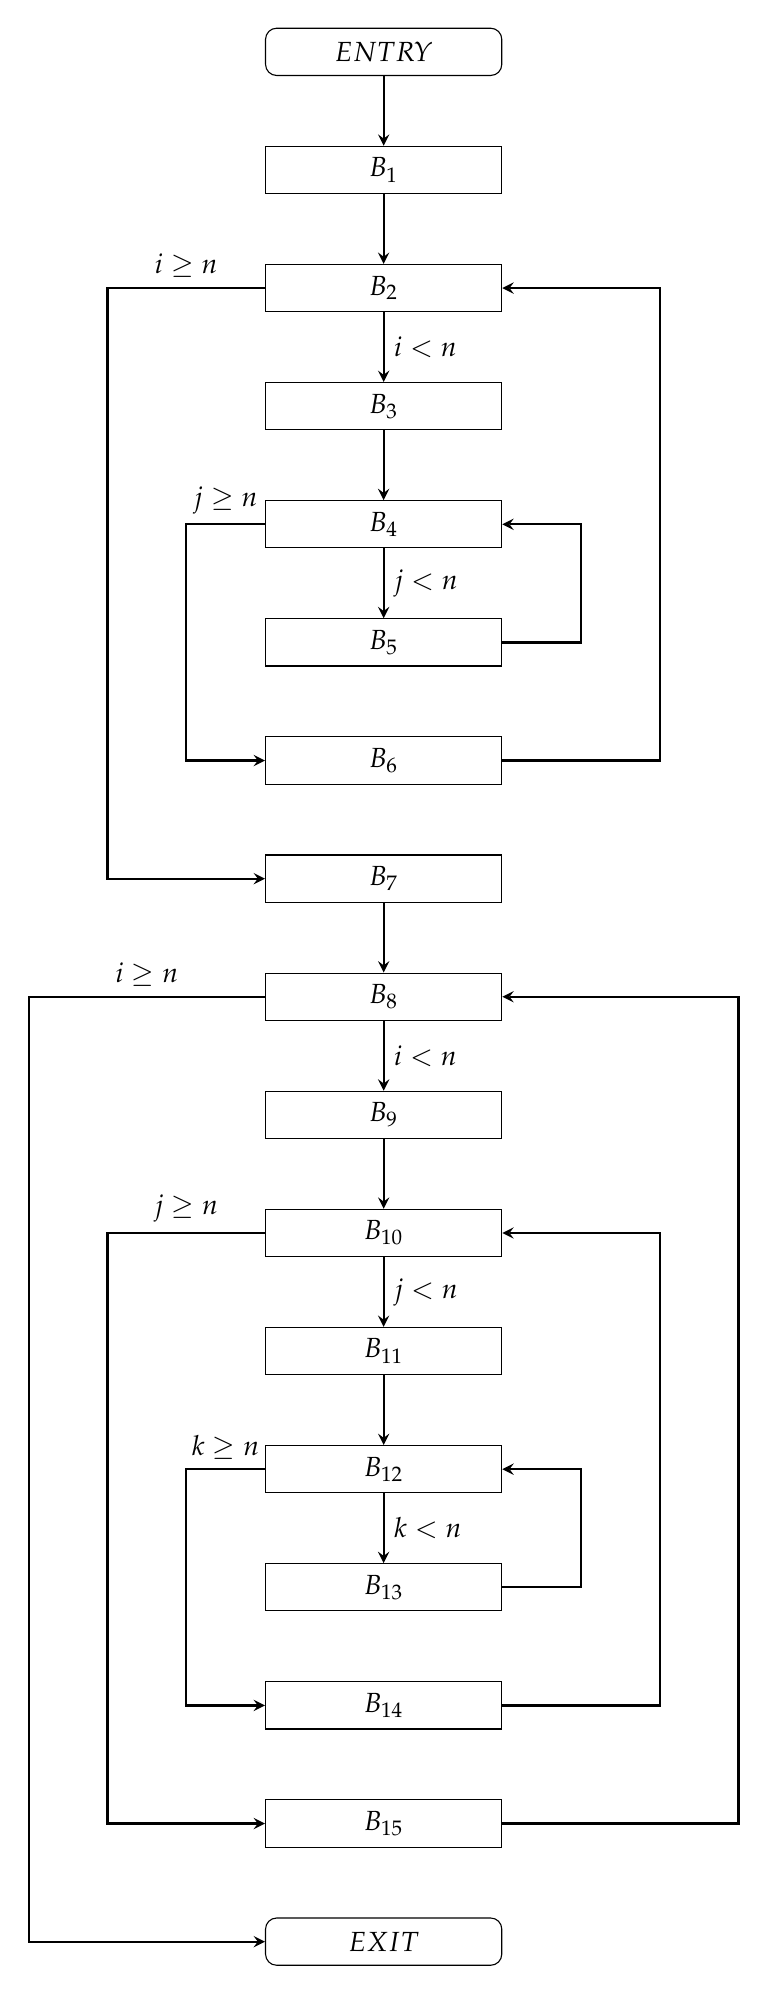
\begin{tikzpicture}[node distance=1.5cm]
	\tikzstyle{be} = [rectangle, rounded corners,minimum width=3cm, minimum height=0.6cm, draw=black]
	\tikzstyle{node} = [rectangle, minimum width=3cm, minimum height=0.6cm,draw=black]
\tikzstyle{arrow} = [thick,->,>=stealth]
  \node(entry)[be] {$ENTRY$};
  \node(b1)[node, below of = entry] {$B_1$};
  \node(b2)[node, below of = b1] {$B_2$};
  \node(b3)[node, below of = b2] {$B_3$};
  \node(b4)[node, below of = b3] {$B_4$};
  \node(b5)[node, below of = b4] {$B_5$};
  \node(b6)[node, below of = b5] {$B_6$};
  \node(b7)[node, below of = b6] {$B_7$};
  \node(b8)[node, below of = b7] {$B_8$};
  \node(b9)[node, below of = b8] {$B_9$};
  \node(b10)[node, below of = b9] {$B_{10}$};
  \node(b11)[node, below of = b10] {$B_{11}$};
  \node(b12)[node, below of = b11] {$B_{12}$};
  \node(b13)[node, below of = b12] {$B_{13}$};
  \node(b14)[node, below of = b13] {$B_{14}$};
  \node(b15)[node, below of = b14] {$B_{15}$};
  \node(exit) [be, below of = b15] {$EXIT$};

  \draw [arrow] (entry) -- (b1);
  \draw [arrow] (b1) -- (b2);
  \draw [arrow] (b2) --node[right]{$i <n$} (b3);
  \draw [arrow] (b3) -- (b4);
  \draw [arrow] (b4) --node[right]{$j<n$} (b5);
  \draw [arrow] (b7) -- (b8);
  \draw [arrow] (b8) --node[right]{$i < n$} (b9);
  \draw [arrow] (b9) -- (b10);
  \draw [arrow] (b10) --node[right]{$j <n$} (b11);
  \draw [arrow] (b11) -- (b12);
  \draw [arrow] (b12) --node[right]{$k <n$} (b13);
  \draw [arrow] (b2)--node[above]{$i\ge n$}($(b2.west) + (-2,0)$) |-(b7);
  \draw [arrow] (b4)--node[above]{$j\ge n$}($(b4.west) + (-1,0)$) |-(b6);
  \draw [arrow] (b6)--($(b6.east) + (2,0)$) |-(b2);
  \draw [arrow] (b5)--($(b5.east) + (1,0)$) |-(b4);
  \draw [arrow] (b12)--node[above]{$k \ge n$}($(b12.west) + (-1,0)$) |-(b14);
  \draw [arrow] (b10)--node[above]{$j\ge n$}($(b10.west) + (-2,0)$) |-(b15);
  \draw [arrow] (b8)--node[above]{$i \ge n$}($(b8.west) + (-3,0)$) |-(exit);
  \draw [arrow] (b13)--($(b13.east) + (1,0)$) |-(b12);
  \draw [arrow] (b14)--($(b14.east) + (2,0)$) |-(b10);
  \draw [arrow] (b15)--($(b15.east) + (3,0)$) |-(b8);
\end{tikzpicture}
\end{figure}

$3)$流图中的循环有:
\begin{align*}
  &\{B_2, B_3, B_4, B_5, B_6\}\\
  &\{B_4, B_5\}\\
  &\{B_8,B_9, B_{10}, B_{11}, B_{12}, B_{13}, B_{14}, B_{15}\}\\
  &\{B_{10}, B_{11}, B_{12}, B_{13}, B_{14}\}\\
  &\{B_{14}, B_{15}\}
\end{align*}

$8.5.1\&2$ 解:构造的$DAG$如下:
\begin{figure}[H]
  \centering
  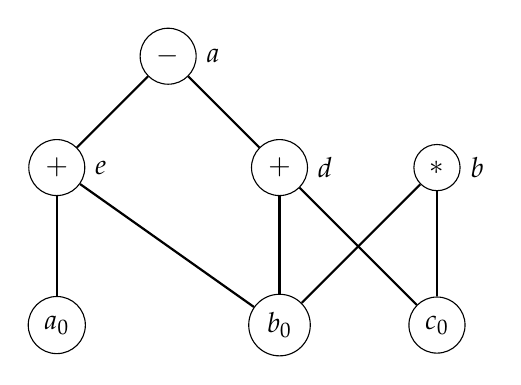
\begin{tikzpicture}[node distance = 2cm]
	\tikzstyle{nn} = [circle,draw = black]
\tikzstyle{line} = [thick,>=stealth]
	\node(a)[nn, label = right:$a$]  {$-$};
	\node(e)[nn, label = right:$e$, below left of= a] {$+$};
	\node(d)[nn, label = right:$d$, below right of = a]  {$+$};
	\node(b)[nn, label = right:$b$, right of = d] {$*$};
	\node(a0) [nn, below of = e] {$a_0$};
	\node(b0)[nn, below of = d] {$b_0$};
	\node(c0)[nn, below of = b]  {$c_0$};
	\draw[line](a) -- (e);
	\draw[line](a) --(d);
	\draw[line](e) --(a0);
	\draw[line](e) --(b0);
	\draw[line](d) --(b0);
	\draw[line](d) --(c0);
	\draw[line](b) --(b0);
	\draw[line](b) --(c0);
  \end{tikzpicture}
\end{figure}

当只有$a$在基本块出口活跃时,代码可简化为:
\begin{lstlisting}
d = b + c;
e = a + b;
a = e - d;
\end{lstlisting}
\end{document}


